% -*- coding: utf-8 -*-
% Шаблон отчета для свободной оптимизации периода P с оценкой погрешностей (Hessian)
\documentclass[12pt,a4paper]{article}

\usepackage{iftex}
\ifPDFTeX
  \usepackage[utf8]{inputenc}
  \usepackage[T2A]{fontenc}
  \usepackage[russian]{babel}
\else
  \usepackage{fontspec}
  \usepackage[russian]{babel}
  \setmainfont{Arial}
\fi

\usepackage{amsmath,amssymb}
\usepackage{graphicx}
\usepackage{booktabs}
\usepackage{geometry}
\geometry{top=2cm,bottom=2cm,left=2cm,right=2cm}
\usepackage{hyperref}
\usepackage{float}
\usepackage{caption}

\graphicspath{{../images/}{docs/images/}{images/}{../../docs/images/}}

\title{Аналитический отчет (Свободный период): Моделирование и анализ погрешностей THz-TDS}
\author{Автоматический анализатор THz-Unified-Optimizer}
\date{\today}

\begin{document}

\maketitle

\tableofcontents
\newpage

\section{Введение}
В данном отчете представлены результаты подгонки комплексной 2D-модели Бланко с размороженным шагом решетки $P$ и оценкой погрешностей всех параметров на основе вычисления численного Гессиана в точке минимума целевой функции.

Оптимизация проводилась на двух наиболее стабильных датасетах с ограничениями:
\begin{itemize}
    \item Шаг решетки $P \in [14.5, 17.5]$ мкм.
    \item Диаметр проволоки $D \in [4.8, 6.2]$ мкм.
\end{itemize}

\section{Результаты оптимизации и анализ погрешностей (Гессиан)}
В таблице \ref{tab:params} приведены оптимальные параметры, полученные для каждой из надежных серий, а также для глобального усреднения, с соответствующими погрешностями $\pm \sigma$, вычисленными как квадратный корень из диагональных элементов ковариационной матрицы $\Sigma = \frac{2 L_{min}}{M} H^{-1}$.

\begin{table}[H]
\centering
\caption{Оптимальные параметры и их погрешности ($\pm \sigma$), полученные методом Гессиана.}
\label{tab:params}
\begin{tabular}{lccc}
\toprule
Параметр & Серия \texttt{356att} & Серия \texttt{series3} & Глобальное усреднение \\
\midrule
$P$ (мкм)           & [Плейсхолдер: $P \pm \sigma_P$] & [Плейсхолдер: $P \pm \sigma_P$] & [Плейсхолдер: $P \pm \sigma_P$] \\
$D$ (мкм)           & [Плейсхолдер: $D \pm \sigma_D$] & [Плейсхолдер: $D \pm \sigma_D$] & [Плейсхолдер: $D \pm \sigma_D$] \\
$\theta_{offset}$ ($^\circ$) & [Плейсхолдер: $\theta \pm \sigma_\theta$] & [Плейсхолдер: $\theta \pm \sigma_\theta$] & [Плейсхолдер: $\theta \pm \sigma_\theta$] \\
$loss\_factor$      & [Плейсхолдер: $L \pm \sigma_L$] & [Плейсхолдер: $L \pm \sigma_L$] & [Плейсхолдер: $L \pm \sigma_L$] \\
$\gamma$            & [Плейсхолдер: $\gamma \pm \sigma_\gamma$] & [Плейсхолдер: $\gamma \pm \sigma_\gamma$] & [Плейсхолдер: $\gamma \pm \sigma_\gamma$] \\
$\tau_{ps}$ (пс)    & [Плейсхолдер: $\tau \pm \sigma_\tau$] & [Плейсхолдер: $\tau \pm \sigma_\tau$] & [Плейсхолдер: $\tau \pm \sigma_\tau$] \\
\midrule
Минимум Loss ($L_{min}$) & [Плейсхолдер] & [Плейсхолдер] & [Плейсхолдер] \\
Число точек ($M$)    & [Плейсхолдер] & [Плейсхолдер] & [Плейсхолдер] \\
\bottomrule
\end{tabular}
\end{table}

\section{Сравнение экспериментальных точек с теорией}
\subsection{Серия 356att}
\begin{figure}[H]
    \centering
    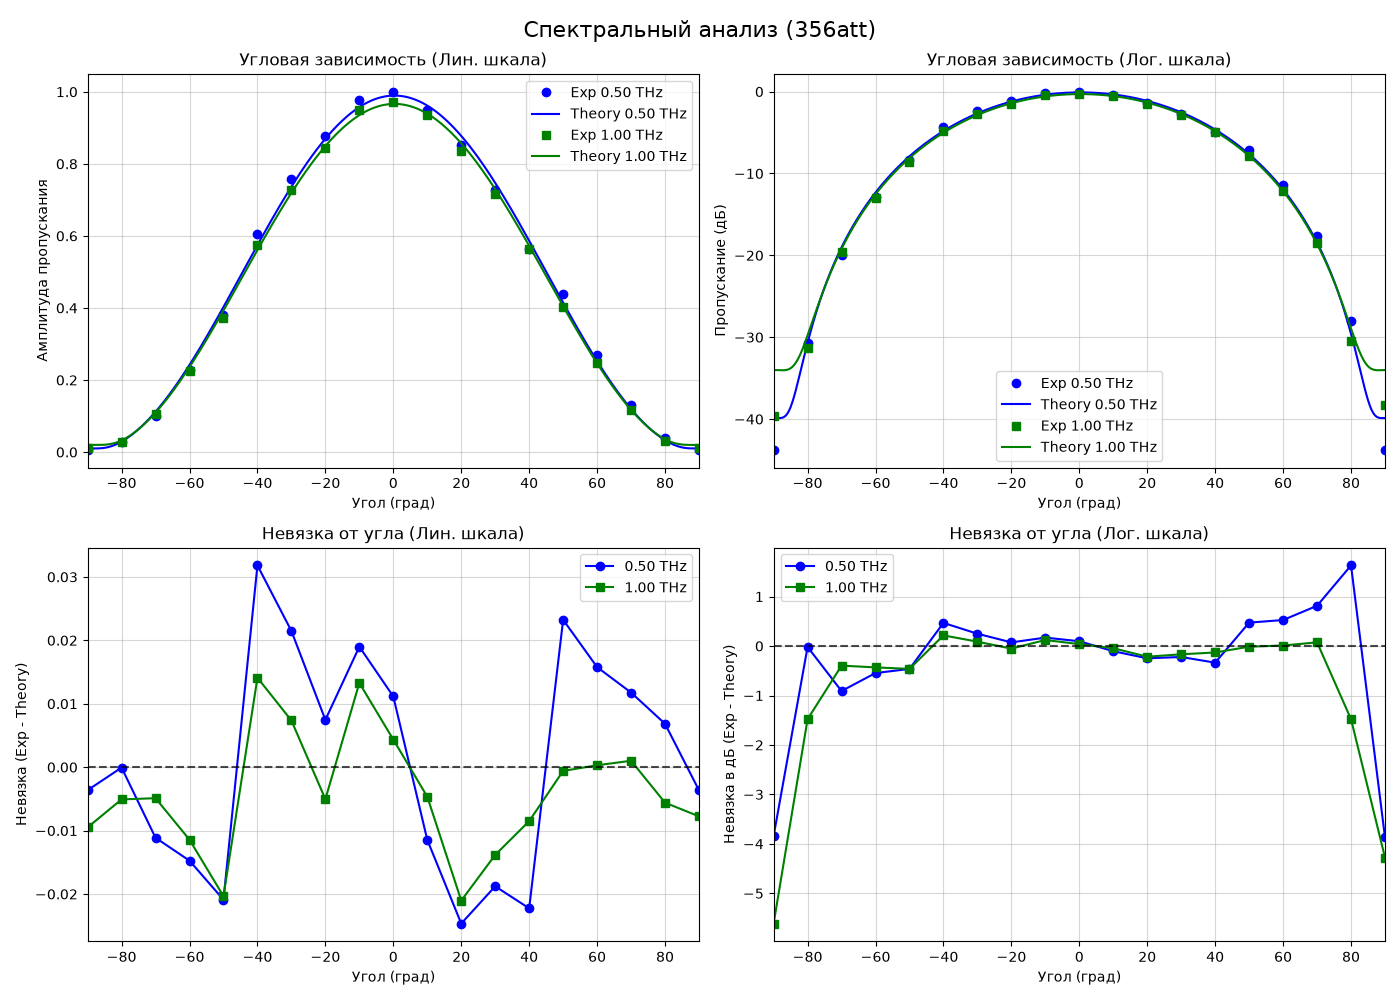
\includegraphics[width=0.48\textwidth]{grid_spectral_356att.png}
    
\includegraphics[width=0.48\textwidth]{grid_integral_356att.png}
    \caption{356att: спектральный анализ (слева) и интегральный метод (справа).}
\end{figure}

\subsection{Серия series3}
\begin{figure}[H]
    \centering
    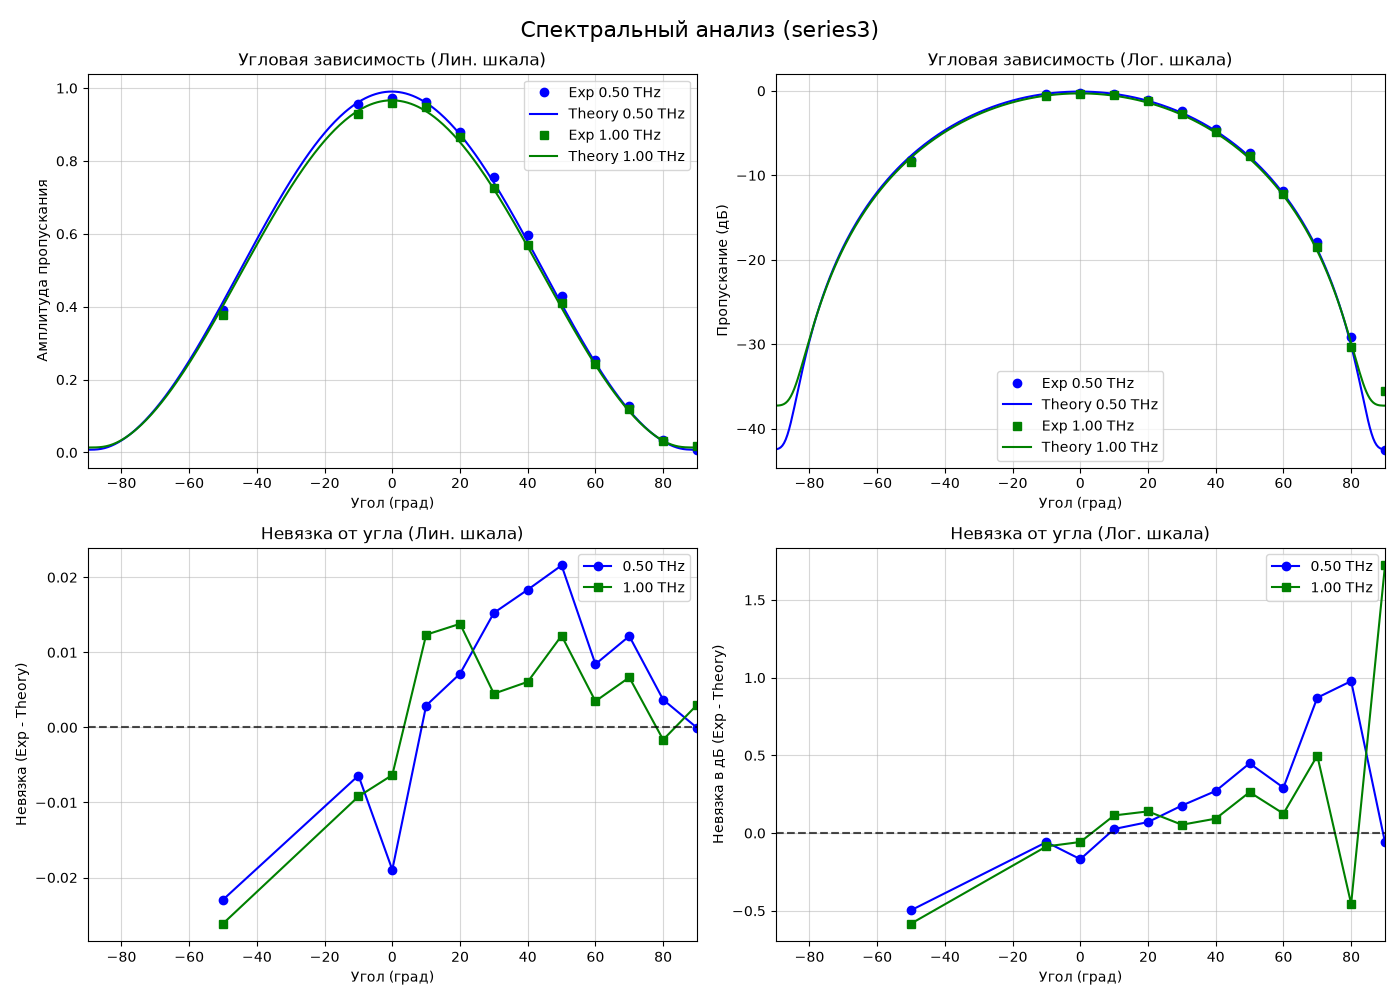
\includegraphics[width=0.48\textwidth]{grid_spectral_series3.png}
    
\includegraphics[width=0.48\textwidth]{grid_integral_series3.png}
    \caption{series3: спектральный анализ (слева) и интегральный метод (справа).}
\end{figure}

\section{Комплексный анализ невязок и корреляций}
[Здесь будет приведено описание невязок для оптимизации со свободным периодом $P$.]

\section{Заключение}
Свободный подбор шага $P$ в физически обоснованных границах позволил дополнительно уточнить эффективные параметры решеток. Малые значения доверительных интервалов $\sigma$ подтверждают высокую устойчивость найденного глобального минимума целевой функции.

\end{document}
